Quantum computing is a rapidly evolving field that has the potential to revolutionize the way we process information. Unlike classical computers, which use bits to represent information, quantum computers use quantum bits or qubits. Due to quantum superposition and entanglement, qubits can exist in multiple states simultaneously, allowing quantum computers to perform certain calculations much faster than classical computers. These algorithms include Grover's search algorithm \cite{grover1996fast, long2001grover}, Shor's factoring algorithm \cite{shor1994algorithms} and HHL linear equations solving algorithm \cite{harrow2009quantum}. In recent years, the development of quantum computing chips has been relatively rapid. IBM has successively launched its 433-bit Osprey quantum chip \cite{ibm2022osprey} and 1121-bit Condor quantum chip \cite{castelvecchi2023ibm}. Google also demonstrate the quantum supremacy on 53-bit Sycamore quantum chip \cite{arute2019quantum}. The 66-bit programmable quantum computing chip Zuchongzhi-2 \cite{wu2021strong} has also been released in China. How to use these quantum chips efficiently has become an increasingly important research topic.

Currently, we are still in the NISQ quantum computing stage \cite{preskill2018quantum}, and the number of qubits in quantum computers is still relatively small with relatively large qubit noise. Therefore, it is particularly important to use classical hardware, such as CPUs, GPUs, and Ascend, to perform quantum simulation. With the quantum simulator, we can quickly develop and verify quantum algorithms. At the same time, we can also use the quantum simulator to verify the correctness of the quantum chip or assist in completing the error mitigation of the current noisy quantum chip.

In the NISQ stage, a type of variational quantum algorithm \cite{Peruzzo2014Peruzzo2014,cerezo2021variational} called quantum-classical hybrid variational algorithm may demonstrate superior practical value. These algorithms have a certain resistance to noise, including the variational quantum eigensolver for simulating chemical molecules \cite{mcardle2020quantum,cao2019quantum,yeter2020practical,fan2023circuit}, quantum approximate optimization algorithm \cite{farhi2014quantum,PhysRevResearch.4.013141} for solving combinatorial optimization problems, and quantum machine learning algorithm \cite{benedetti2019parameterized,biamonte2017quantum,das2019machine} for processing classification and pattern generation. According to the principle of variational algorithms, variational quantum algorithms use classical optimizers to continuously adjust the parameters in the variational quantum circuit to make the quantum system output as close as possible to the expected target, thereby achieving the purpose of optimization learning.

Based on the above discussion, here we announce a new hybrid quantum-classical programming framework called MindSpore Quantum (\MindQuantum). Compared to current quantum framework such as QuEST \cite{jones2019quest}, QPanda \cite{dou2022qpanda}, TensorCircuit \cite{zhang2023tensorcircuit}, Qulacs \cite{suzuki2021qulacs}, TensorFlow Quantum \cite{broughton2020tensorflow}, Yao \cite{luo2020yao}, Intel Quantum Simulator \cite{guerreschi2020intel}, and PennyLane \cite{bergholm2018pennylane}, \MindQuantum\ provides a simple, user-friendly, and efficient quantum programming framework that supports the construction, simulation and real chip based execution of quantum circuits. By integrating with MindSpore, it enables fast development and training of hybrid quantum-classical algorithms. Fig.~\ref{fig:framework} illustrates the overall architecture of \MindQuantum.

\definecolor{c8adacd}{RGB}{138,218,205}
\definecolor{ce8f8f3}{RGB}{232,248,243}
\definecolor{cffc46d}{RGB}{255,196,109}
\definecolor{cf2f2f2}{RGB}{220,220,220}
\definecolor{c6de1ff}{RGB}{109,225,255}
\definecolor{caffaeb}{RGB}{175,250,235}
\definecolor{c0157b4}{RGB}{1,87,180}
\def \globalscale {1.000000}
\begin{figure*}
    \begin{tikzpicture}[scale=0.6, every node/.append style={scale=\globalscale}, inner sep=0pt, outer sep=0pt]
        % Basic Component
        \path[draw=black,line width=0.0794cm] (0.0397, 29.1174) rectangle (29.2232, 17.8991);
        \node[align=center, font=\bfseries] at (14.63145, 28.5174) {Basic Component};

        \path[fill=c8adacd, draw] (0.4895, 28.0061) rectangle (7.3686, 27.0272);
        \node[align=center] at (3.92905, 27.51665) {Quantum Gate};


        \path[fill=ce8f8f3] (0.4763, 26.8023) rectangle (7.3819, 18.2563);
        \node[draw=none] at (4.2, 25) {
            \begin{minipage}{0.3\textwidth}
                \begin{itemize}
                    \item Fixed gate
                    \item Parameterized gate
                    \item Any control on any gate
                    \item Noise channel
                \end{itemize}
            \end{minipage}
        };
        \path[fill=white,rounded corners=0.6879cm] (0.926, 22.8865) rectangle (6.9321, 18.6796);


        \path[fill=c8adacd, draw] (7.6332, 28.0061) rectangle (14.4859, 27.0272);
        \node[align=center] at (11.05955, 27.51665) {Quantum Circuit};

        \path[fill=ce8f8f3] (7.62, 26.8023) rectangle (14.5256, 18.2563);
        \node[draw=none] at (11.3437, 25.5) {
            \begin{minipage}{0.3\textwidth}
                \begin{itemize}
                    \item Append operator
                    \item $+=$ operator
                    \item Chain rule
                \end{itemize}
            \end{minipage}
        };
        \path[fill=white,rounded corners=0.6879cm] (8.0698, 22.8865) rectangle (14.0758, 18.6796);

        \path[fill=c8adacd, draw] (14.777, 28.0061) rectangle (21.6561, 27.0272);
        \node[align=center] at (18.21655, 27.51665) {Parameter Resolver};
        \path[fill=ce8f8f3] (14.7638, 26.8023) rectangle (21.6694, 18.2563);
        \node[draw=none] at (18.4875, 25.9) {
            \begin{minipage}{0.3\textwidth}
                \begin{itemize}
                    \item Fine tuning
                    \item Arithmetic calculation
                \end{itemize}
            \end{minipage}
        };
        \path[fill=white,rounded corners=0.6879cm] (15.2135, 22.8865) rectangle (21.2196, 18.6796);

        \path[fill=c8adacd, draw] (21.9207, 28.0061) rectangle (28.7734, 27.0272);
        \node[align=center] at (25.34705, 27.51665) {Observable};
        \path[fill=ce8f8f3] (21.9075, 26.8023) rectangle (28.8131, 18.2563);
        \node[draw=none] at (25.6312, 25) {
            \begin{minipage}{0.3\textwidth}
                \begin{itemize}
                    \item Hamiltonian
                    \item QubitOperator
                    \item FermionOperator
                    \item Transform
                \end{itemize}
            \end{minipage}
        };
        \path[fill=white,rounded corners=0.6879cm] (22.3573, 22.8865) rectangle (28.3633, 18.6796);
        \node at (3.92905, 20.78305) {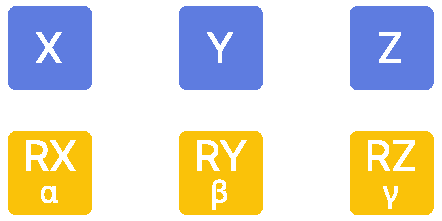
\includegraphics[scale=0.4]{images/1_1_1.pdf}};
        \node at (11.07285, 20.78305) {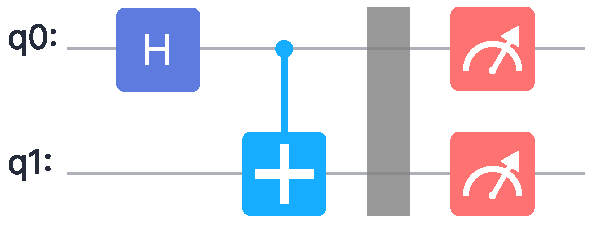
\includegraphics[scale=0.35]{images/1_1_2.pdf}};
        \node at (18.21665, 21.18305){\begin{lstlisting}[numbers=none, backgroundcolor=]
a, b = np.pi, 0.5
ParameterResolver({
 'a': a, 'b': b
})\end{lstlisting}};

        \node[align=center] at (18.21665, 19.68305) {\textcolor{blue}{$\pi * a+ 1 / 2 * b$}};
        \node at (25.36045, 21.18305-0.2){\begin{lstlisting}[numbers=none, backgroundcolor=]
o = QubitOperator(
 'X0 Y1', 'a'
) + QubitOperator(
 'Z2', np.sqrt(2)
)
        \end{lstlisting}};
        \node[align=center] at (25.36045, 19.68305-0.2) {\textcolor{blue}{$aX_0Y_1 + \sqrt{2}Z_2$}};

        % NISQ
        \path[draw=black,line width=0.0794cm] (0.0397, 17.608) rectangle (14.4595, 10.2791);
        \node[align=center, font=\bfseries] at (7.2496, 17.008) {NISQ Algorithm};

        \path[fill=cffc46d,draw] (0.5159, 16.047) rectangle (6.9453, 14.7505);
        \node[align=center] at (3.7306, 15.39875) {Ansatz Library};

        \path[draw=black] (0.5159, 14.7241) rectangle (6.9453, 10.5436);

        \path[fill=cffc46d,draw] (7.62, 16.0602) rectangle (14.0758, 14.7373);
        \node[align=center] at (10.8479, 15.39875) {VQE};

        \path[fill=cffc46d, draw] (7.62, 13.9435) rectangle (14.0758, 12.6206);
        \node[align=center] at (10.8479, 13.28205) {QAOA};

        \path[fill=cffc46d, draw] (7.62, 11.8269) rectangle (14.0758, 10.504);
        \node[align=center] at (10.8479, 11.16545) {QNN};
        \node at (3.7306, 12.58205) {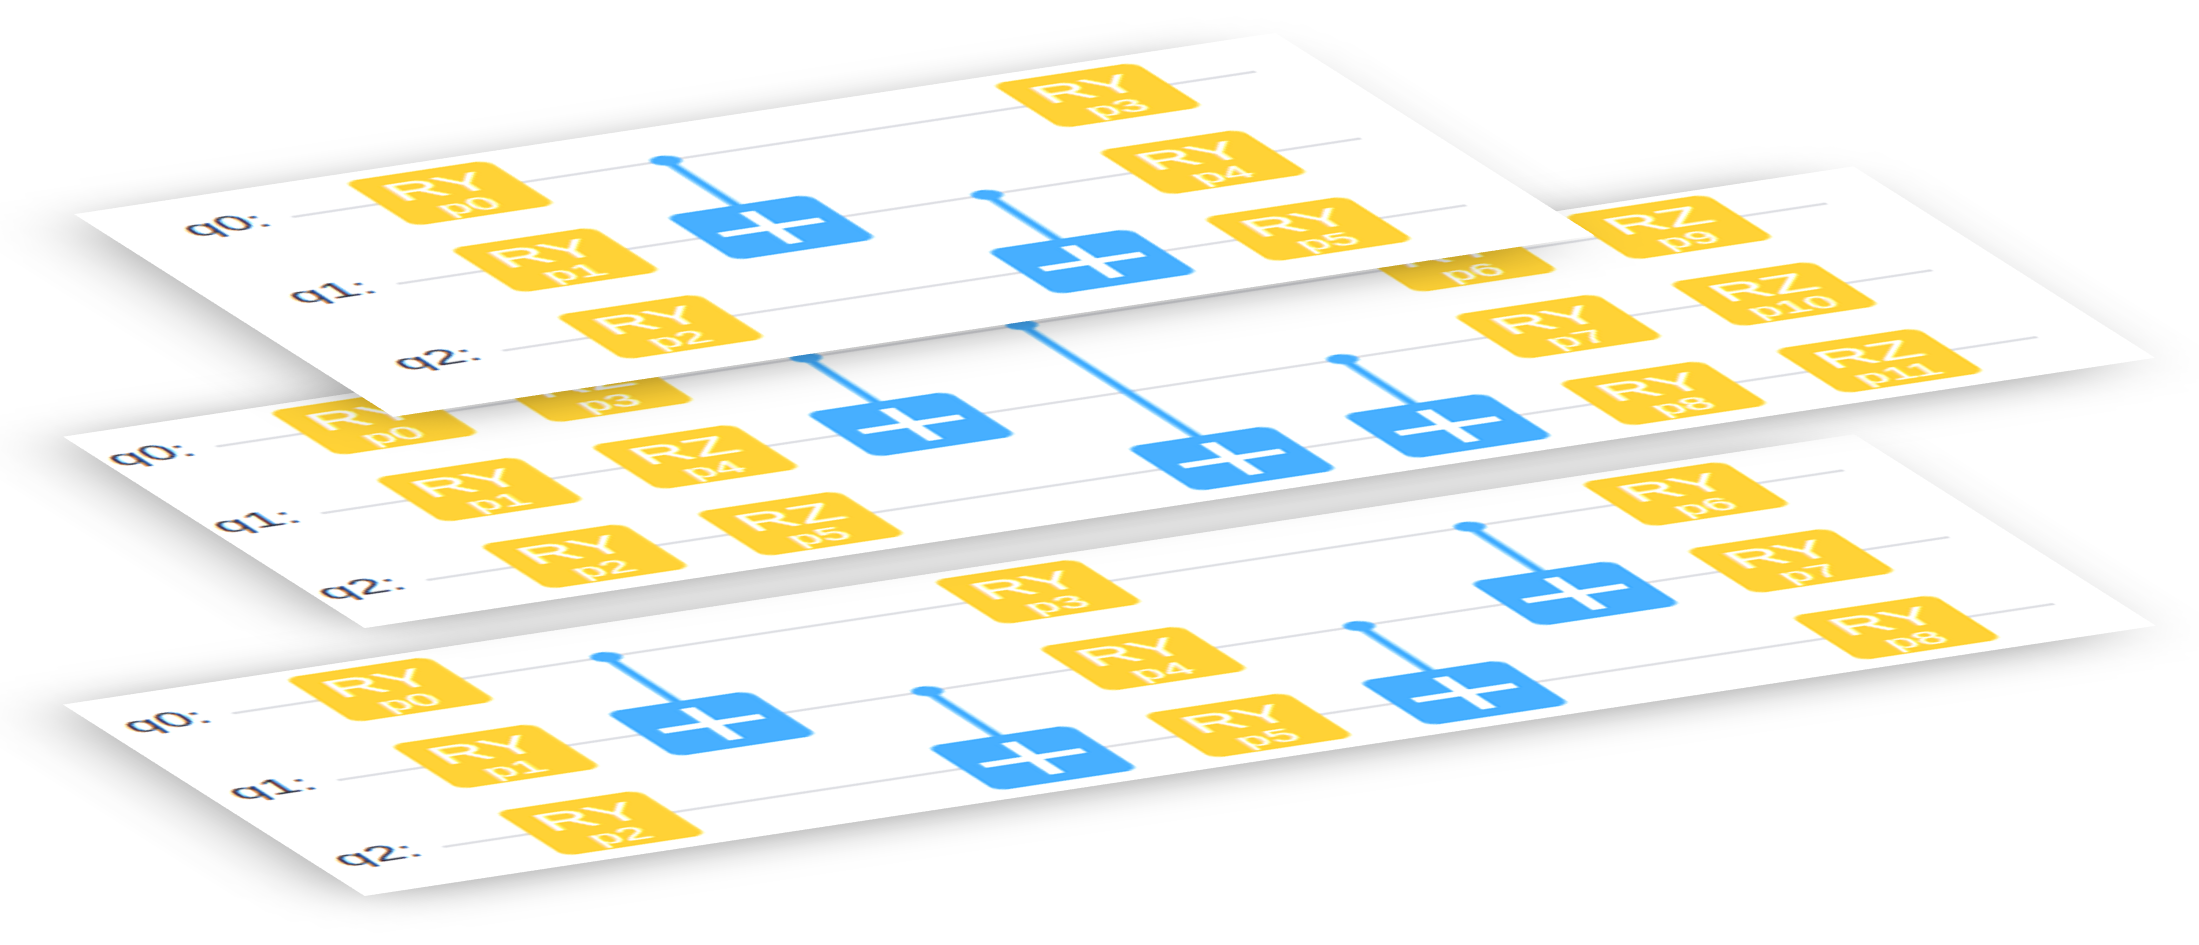
\includegraphics[scale=0.065]{images/1_1_4.jpeg}};


        % Compiler
        \path[draw=black,line width=0.0794cm] (14.8034, 17.608) rectangle (29.2232, 10.2791);
        \node[align=center, font=\bfseries] at (22.0133, 17.008) {Compiler Algorithm};

        \path[fill=cffc46d,draw] (19.7379, 15.2929) rectangle (28.3633, 13.97);
        \node[align=center] at (24.0506, 14.63145) {DAG based circuit compiler};

        \path[fill=cffc46d,draw] (19.7379, 12.4883) rectangle (28.3633, 11.1654);
        \node[align=center] at (24.0506, 11.82685) {Qubit Mapping};
        \node at (17.2506, 13.22915) {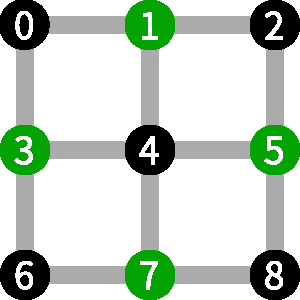
\includegraphics[scale=0.5]{images/1_1_3.pdf}};

        % simulator
        \path[draw=black,line width=0.0794cm] (0.0397, 9.8822) rectangle (14.4595, 3.2941);
        \node[align=center, font=\bfseries] at (7.2496, 9.2822) {Quantum Simulator};

        \path[fill=c6de1ff] (0.4895, 8.5328) rectangle (14.0626, 7.2364);
        \node[align=center] at (7.2496, 7.8846) {Core Simulation Algorithm};

        \path[fill=caffaeb] (0.4763, 6.9585) rectangle (14.0758, 3.5719);
        \node[draw=none] at (5.7, 5.2415) {
            \begin{minipage}{0.4\textwidth}
                \begin{itemize}
                    \item Evolution of Circuit
                    \item Sampling Measurement
                    \item Expectation of Observable
                    \item Gradient calculation in batch mode
                \end{itemize}
            \end{minipage}
        };

        % cpu_gpu
        \path[draw=black,line width=0.0794cm] (0.0661, 2.8972) rectangle (14.4859, 0.0397);
        \node[align=center, font=\bfseries] at (7.276,2.2972) {Policy Detail};

        \path[fill=c0157b4] (0.2646, 1.7992) rectangle (4.6038, 0.2117);
        \node[align=center,text=white] at (2.4342,1.00545) {X86(AVX)};

        \path[fill=c0157b4] (5.0271, 1.7992) rectangle (9.3663, 0.2117);
        \node[align=center,text=white] at (7.1967,1.00545) {GPU(CUDA)};

        \path[fill=c0157b4] (9.7896, 1.7992) rectangle (14.1288, 0.2117);
        \node[align=center,text=white] at (11.9592,1.00545) {Ascend(NENO)};


        % provider
        \path[fill=cf2f2f2] (14.8034, 9.8822) rectangle (29.2232, 3.2941);
        \path[draw=black,line width=0.0794cm,dash pattern=on 0.1588cm off 0.1588cm] (14.8034, 9.8822) rectangle (29.2232, 3.2941);
        \node[align=center, font=\bfseries] at (22.0133, 6.58815) {Backend Provider};

        % QPU
        \path[fill=cf2f2f2] (14.8034, 2.8972) rectangle (29.2232, 0.0397);
        \path[draw=black,line width=0.0794cm,dash pattern=on 0.1588cm off 0.1588cm] (14.8034, 2.8972) rectangle (29.2232, 0.0397);
        \node[align=center, font=\bfseries] at (22.0133, 1.46845) {QPU};

    \end{tikzpicture}
    \caption{The framework of \MindQuantum}
    \label{fig:framework}
\end{figure*}


\begin{description}
    \item[First layer] This layer represents the fundamental building blocks of the framework. We provide various quantum gates and convenient ways to construct quantum circuits. To support variational quantum algorithms, we also offer a parameter resolver that converts certain quantum gates into variational ones. Additionally, we provide the capability to describe various observables.
    \item[Second layer] This layer is the algorithm layer, which includes general quantum algorithms and variational quantum algorithms in the NISQ era. Furthermore, this layer encompasses quantum compilation algorithms that compile and map quantum circuits to quantum chips.
    \item[Third layer] This layer is the execution layer, which is divided into a quantum simulator and a quantum chip backend provider depending on the hardware used for execution. In the quantum simulator, we design high-performance simulation logic tailored for CPU, GPU, and Ascend architectures, allowing for flexible switching between single-precision and double-precision simulation modes.
\end{description}

The arrangement of this whitepaper is as follows: In Chapter \hyperref[sec:elements]{\ref*{sec:elements}}, we will introduce the fundamental elements in \MindQuantum\ for constructing quantum circuits and observables. Chapter \hyperref[sec:backend]{\ref*{sec:backend}} will provide a comprehensive demonstration of the usage methods for the quantum simulator. In Chapter \hyperref[sec:toolbox]{\ref*{sec:toolbox}}, we will discuss the modules in \MindQuantum\ that are relevant to variational quantum algorithms, including various types of variational quantum circuits and methods for solving gradients of variational quantum circuits. Chapter \hyperref[sec:applications]{\ref*{sec:applications}} will showcase the reproduction of cutting-edge research results in the current academic community using \MindQuantum. Chapter \hyperref[sec:qupack]{\ref*{sec:qupack}} will introduce the quantum acceleration engine, QuPack, which can significantly enhance quantum simulation efficiency in certain scenarios. In Chapter \hyperref[sec:benchmark]{\ref*{sec:benchmark}}, we will benchmark the performance of \MindQuantum\ against some industry-standard quantum computing frameworks in different scenarios. Chapter \hyperref[sec:chip]{\ref*{sec:chip}} will explain how to utilize \MindQuantum\ to run quantum algorithms on real quantum chips. We will summarize the whole paper in Chapter \hyperref[sec:summary]{\ref*{sec:summary}}. Finally, in Chapter \hyperref[sec:acknowledgement]{\ref*{sec:acknowledgement}}, we will express our gratitude to all those who have contributed to \MindQuantum\ and those who are willing to use \MindQuantum\ in their research.
